% Options for packages loaded elsewhere
\PassOptionsToPackage{unicode}{hyperref}
\PassOptionsToPackage{hyphens}{url}
\PassOptionsToPackage{dvipsnames,svgnames,x11names}{xcolor}
%
\documentclass[
  letterpaper,
  DIV=11,
  numbers=noendperiod,
  oneside]{scrreprt}

\usepackage{amsmath,amssymb}
\usepackage{iftex}
\ifPDFTeX
  \usepackage[T1]{fontenc}
  \usepackage[utf8]{inputenc}
  \usepackage{textcomp} % provide euro and other symbols
\else % if luatex or xetex
  \usepackage{unicode-math}
  \defaultfontfeatures{Scale=MatchLowercase}
  \defaultfontfeatures[\rmfamily]{Ligatures=TeX,Scale=1}
\fi
\usepackage{lmodern}
\ifPDFTeX\else  
    % xetex/luatex font selection
\fi
% Use upquote if available, for straight quotes in verbatim environments
\IfFileExists{upquote.sty}{\usepackage{upquote}}{}
\IfFileExists{microtype.sty}{% use microtype if available
  \usepackage[]{microtype}
  \UseMicrotypeSet[protrusion]{basicmath} % disable protrusion for tt fonts
}{}
\makeatletter
\@ifundefined{KOMAClassName}{% if non-KOMA class
  \IfFileExists{parskip.sty}{%
    \usepackage{parskip}
  }{% else
    \setlength{\parindent}{0pt}
    \setlength{\parskip}{6pt plus 2pt minus 1pt}}
}{% if KOMA class
  \KOMAoptions{parskip=half}}
\makeatother
\usepackage{xcolor}
\usepackage[left=1in,marginparwidth=2.0666666666667in,textwidth=4.1333333333333in,marginparsep=0.3in]{geometry}
\setlength{\emergencystretch}{3em} % prevent overfull lines
\setcounter{secnumdepth}{5}
% Make \paragraph and \subparagraph free-standing
\makeatletter
\ifx\paragraph\undefined\else
  \let\oldparagraph\paragraph
  \renewcommand{\paragraph}{
    \@ifstar
      \xxxParagraphStar
      \xxxParagraphNoStar
  }
  \newcommand{\xxxParagraphStar}[1]{\oldparagraph*{#1}\mbox{}}
  \newcommand{\xxxParagraphNoStar}[1]{\oldparagraph{#1}\mbox{}}
\fi
\ifx\subparagraph\undefined\else
  \let\oldsubparagraph\subparagraph
  \renewcommand{\subparagraph}{
    \@ifstar
      \xxxSubParagraphStar
      \xxxSubParagraphNoStar
  }
  \newcommand{\xxxSubParagraphStar}[1]{\oldsubparagraph*{#1}\mbox{}}
  \newcommand{\xxxSubParagraphNoStar}[1]{\oldsubparagraph{#1}\mbox{}}
\fi
\makeatother

\usepackage{color}
\usepackage{fancyvrb}
\newcommand{\VerbBar}{|}
\newcommand{\VERB}{\Verb[commandchars=\\\{\}]}
\DefineVerbatimEnvironment{Highlighting}{Verbatim}{commandchars=\\\{\}}
% Add ',fontsize=\small' for more characters per line
\usepackage{framed}
\definecolor{shadecolor}{RGB}{241,243,245}
\newenvironment{Shaded}{\begin{snugshade}}{\end{snugshade}}
\newcommand{\AlertTok}[1]{\textcolor[rgb]{0.68,0.00,0.00}{#1}}
\newcommand{\AnnotationTok}[1]{\textcolor[rgb]{0.37,0.37,0.37}{#1}}
\newcommand{\AttributeTok}[1]{\textcolor[rgb]{0.40,0.45,0.13}{#1}}
\newcommand{\BaseNTok}[1]{\textcolor[rgb]{0.68,0.00,0.00}{#1}}
\newcommand{\BuiltInTok}[1]{\textcolor[rgb]{0.00,0.23,0.31}{#1}}
\newcommand{\CharTok}[1]{\textcolor[rgb]{0.13,0.47,0.30}{#1}}
\newcommand{\CommentTok}[1]{\textcolor[rgb]{0.37,0.37,0.37}{#1}}
\newcommand{\CommentVarTok}[1]{\textcolor[rgb]{0.37,0.37,0.37}{\textit{#1}}}
\newcommand{\ConstantTok}[1]{\textcolor[rgb]{0.56,0.35,0.01}{#1}}
\newcommand{\ControlFlowTok}[1]{\textcolor[rgb]{0.00,0.23,0.31}{\textbf{#1}}}
\newcommand{\DataTypeTok}[1]{\textcolor[rgb]{0.68,0.00,0.00}{#1}}
\newcommand{\DecValTok}[1]{\textcolor[rgb]{0.68,0.00,0.00}{#1}}
\newcommand{\DocumentationTok}[1]{\textcolor[rgb]{0.37,0.37,0.37}{\textit{#1}}}
\newcommand{\ErrorTok}[1]{\textcolor[rgb]{0.68,0.00,0.00}{#1}}
\newcommand{\ExtensionTok}[1]{\textcolor[rgb]{0.00,0.23,0.31}{#1}}
\newcommand{\FloatTok}[1]{\textcolor[rgb]{0.68,0.00,0.00}{#1}}
\newcommand{\FunctionTok}[1]{\textcolor[rgb]{0.28,0.35,0.67}{#1}}
\newcommand{\ImportTok}[1]{\textcolor[rgb]{0.00,0.46,0.62}{#1}}
\newcommand{\InformationTok}[1]{\textcolor[rgb]{0.37,0.37,0.37}{#1}}
\newcommand{\KeywordTok}[1]{\textcolor[rgb]{0.00,0.23,0.31}{\textbf{#1}}}
\newcommand{\NormalTok}[1]{\textcolor[rgb]{0.00,0.23,0.31}{#1}}
\newcommand{\OperatorTok}[1]{\textcolor[rgb]{0.37,0.37,0.37}{#1}}
\newcommand{\OtherTok}[1]{\textcolor[rgb]{0.00,0.23,0.31}{#1}}
\newcommand{\PreprocessorTok}[1]{\textcolor[rgb]{0.68,0.00,0.00}{#1}}
\newcommand{\RegionMarkerTok}[1]{\textcolor[rgb]{0.00,0.23,0.31}{#1}}
\newcommand{\SpecialCharTok}[1]{\textcolor[rgb]{0.37,0.37,0.37}{#1}}
\newcommand{\SpecialStringTok}[1]{\textcolor[rgb]{0.13,0.47,0.30}{#1}}
\newcommand{\StringTok}[1]{\textcolor[rgb]{0.13,0.47,0.30}{#1}}
\newcommand{\VariableTok}[1]{\textcolor[rgb]{0.07,0.07,0.07}{#1}}
\newcommand{\VerbatimStringTok}[1]{\textcolor[rgb]{0.13,0.47,0.30}{#1}}
\newcommand{\WarningTok}[1]{\textcolor[rgb]{0.37,0.37,0.37}{\textit{#1}}}

\providecommand{\tightlist}{%
  \setlength{\itemsep}{0pt}\setlength{\parskip}{0pt}}\usepackage{longtable,booktabs,array}
\usepackage{calc} % for calculating minipage widths
% Correct order of tables after \paragraph or \subparagraph
\usepackage{etoolbox}
\makeatletter
\patchcmd\longtable{\par}{\if@noskipsec\mbox{}\fi\par}{}{}
\makeatother
% Allow footnotes in longtable head/foot
\IfFileExists{footnotehyper.sty}{\usepackage{footnotehyper}}{\usepackage{footnote}}
\makesavenoteenv{longtable}
\usepackage{graphicx}
\makeatletter
\def\maxwidth{\ifdim\Gin@nat@width>\linewidth\linewidth\else\Gin@nat@width\fi}
\def\maxheight{\ifdim\Gin@nat@height>\textheight\textheight\else\Gin@nat@height\fi}
\makeatother
% Scale images if necessary, so that they will not overflow the page
% margins by default, and it is still possible to overwrite the defaults
% using explicit options in \includegraphics[width, height, ...]{}
\setkeys{Gin}{width=\maxwidth,height=\maxheight,keepaspectratio}
% Set default figure placement to htbp
\makeatletter
\def\fps@figure{htbp}
\makeatother
% definitions for citeproc citations
\NewDocumentCommand\citeproctext{}{}
\NewDocumentCommand\citeproc{mm}{%
  \begingroup\def\citeproctext{#2}\cite{#1}\endgroup}
\makeatletter
 % allow citations to break across lines
 \let\@cite@ofmt\@firstofone
 % avoid brackets around text for \cite:
 \def\@biblabel#1{}
 \def\@cite#1#2{{#1\if@tempswa , #2\fi}}
\makeatother
\newlength{\cslhangindent}
\setlength{\cslhangindent}{1.5em}
\newlength{\csllabelwidth}
\setlength{\csllabelwidth}{3em}
\newenvironment{CSLReferences}[2] % #1 hanging-indent, #2 entry-spacing
 {\begin{list}{}{%
  \setlength{\itemindent}{0pt}
  \setlength{\leftmargin}{0pt}
  \setlength{\parsep}{0pt}
  % turn on hanging indent if param 1 is 1
  \ifodd #1
   \setlength{\leftmargin}{\cslhangindent}
   \setlength{\itemindent}{-1\cslhangindent}
  \fi
  % set entry spacing
  \setlength{\itemsep}{#2\baselineskip}}}
 {\end{list}}
\usepackage{calc}
\newcommand{\CSLBlock}[1]{\hfill\break\parbox[t]{\linewidth}{\strut\ignorespaces#1\strut}}
\newcommand{\CSLLeftMargin}[1]{\parbox[t]{\csllabelwidth}{\strut#1\strut}}
\newcommand{\CSLRightInline}[1]{\parbox[t]{\linewidth - \csllabelwidth}{\strut#1\strut}}
\newcommand{\CSLIndent}[1]{\hspace{\cslhangindent}#1}

\KOMAoption{captions}{tableheading}
\makeatletter
\@ifpackageloaded{tcolorbox}{}{\usepackage[skins,breakable]{tcolorbox}}
\@ifpackageloaded{fontawesome5}{}{\usepackage{fontawesome5}}
\definecolor{quarto-callout-color}{HTML}{909090}
\definecolor{quarto-callout-note-color}{HTML}{0758E5}
\definecolor{quarto-callout-important-color}{HTML}{CC1914}
\definecolor{quarto-callout-warning-color}{HTML}{EB9113}
\definecolor{quarto-callout-tip-color}{HTML}{00A047}
\definecolor{quarto-callout-caution-color}{HTML}{FC5300}
\definecolor{quarto-callout-color-frame}{HTML}{acacac}
\definecolor{quarto-callout-note-color-frame}{HTML}{4582ec}
\definecolor{quarto-callout-important-color-frame}{HTML}{d9534f}
\definecolor{quarto-callout-warning-color-frame}{HTML}{f0ad4e}
\definecolor{quarto-callout-tip-color-frame}{HTML}{02b875}
\definecolor{quarto-callout-caution-color-frame}{HTML}{fd7e14}
\makeatother
\makeatletter
\@ifpackageloaded{bookmark}{}{\usepackage{bookmark}}
\makeatother
\makeatletter
\@ifpackageloaded{caption}{}{\usepackage{caption}}
\AtBeginDocument{%
\ifdefined\contentsname
  \renewcommand*\contentsname{Table of contents}
\else
  \newcommand\contentsname{Table of contents}
\fi
\ifdefined\listfigurename
  \renewcommand*\listfigurename{List of Figures}
\else
  \newcommand\listfigurename{List of Figures}
\fi
\ifdefined\listtablename
  \renewcommand*\listtablename{List of Tables}
\else
  \newcommand\listtablename{List of Tables}
\fi
\ifdefined\figurename
  \renewcommand*\figurename{Figure}
\else
  \newcommand\figurename{Figure}
\fi
\ifdefined\tablename
  \renewcommand*\tablename{Table}
\else
  \newcommand\tablename{Table}
\fi
}
\@ifpackageloaded{float}{}{\usepackage{float}}
\floatstyle{ruled}
\@ifundefined{c@chapter}{\newfloat{codelisting}{h}{lop}}{\newfloat{codelisting}{h}{lop}[chapter]}
\floatname{codelisting}{Listing}
\newcommand*\listoflistings{\listof{codelisting}{List of Listings}}
\makeatother
\makeatletter
\makeatother
\makeatletter
\@ifpackageloaded{caption}{}{\usepackage{caption}}
\@ifpackageloaded{subcaption}{}{\usepackage{subcaption}}
\makeatother
\makeatletter
\@ifpackageloaded{sidenotes}{}{\usepackage{sidenotes}}
\@ifpackageloaded{marginnote}{}{\usepackage{marginnote}}
\makeatother
\makeatletter
\@ifpackageloaded{tikz}{}{\usepackage{tikz}}
\makeatother
        \newcommand*\circled[1]{\tikz[baseline=(char.base)]{
          \node[shape=circle,draw,inner sep=1pt] (char) {{\scriptsize#1}};}}  
                  
\newcounter{quartocalloutnteno}
\newcommand{\quartocalloutnte}[1]{\refstepcounter{quartocalloutnteno}\label{#1}}

\ifLuaTeX
  \usepackage{selnolig}  % disable illegal ligatures
\fi
\usepackage{bookmark}

\IfFileExists{xurl.sty}{\usepackage{xurl}}{} % add URL line breaks if available
\urlstyle{same} % disable monospaced font for URLs
\hypersetup{
  pdftitle={Literate programming for the Social, Behavioral, and Management sciences},
  pdfauthor={John Kulas},
  colorlinks=true,
  linkcolor={blue},
  filecolor={Maroon},
  citecolor={Blue},
  urlcolor={Blue},
  pdfcreator={LaTeX via pandoc}}


\title{Literate programming for the Social, Behavioral, and Management
sciences}
\author{John Kulas}
\date{2025-01-01}

\begin{document}
\maketitle

\renewcommand*\contentsname{Table of contents}
{
\hypersetup{linkcolor=}
\setcounter{tocdepth}{2}
\tableofcontents
}

\bookmarksetup{startatroot}

\chapter*{Overview}\label{overview}
\addcontentsline{toc}{chapter}{Overview}

\markboth{Overview}{Overview}

This is a working outline of the curricular syllabus\footnote{and maybe
  eventually ``textbook''-ish content} for a 15-week course on
\href{https://www-cs-faculty.stanford.edu/~knuth/lp.html}{literate
programming} as a workflow framework for I/O Psychologists working in
data science applications. Literate programming reduces the: 1)
occurrence, and 2) consequence of error within work processes.

Traditionally, within the social, behavioral, and management sciences,
your \textbf{analyses} were performed within a secondary
platform\footnote{Excel, GAUSS, SAS, SPSS, STATA, etc\ldots{}} --
\textbf{completely independent} from your primary authoring space (e.g.,
a typewriter, Word, PowerPoint). Literate programming principles
``flip'' this orientation\ldots{} the analyses are primary, and the
\emph{authoring space} is agnostic -- all authoring occurs fully
embedded within the analytical platform.

The primary programming languages accommodated as of
\texttt{r\ format(Sys.time(),\ "\%B\ \%Y")} are:

\begin{itemize}
\tightlist
\item
  R
\item
  Python
\item
  Javascript
\item
  Julia
\end{itemize}

\marginnote{\begin{footnotesize}

\begin{tcolorbox}[enhanced jigsaw, colbacktitle=quarto-callout-note-color!10!white, coltitle=black, rightrule=.15mm, toprule=.15mm, left=2mm, arc=.35mm, colframe=quarto-callout-note-color-frame, opacityback=0, breakable, bottomrule=.15mm, bottomtitle=1mm, opacitybacktitle=0.6, toptitle=1mm, titlerule=0mm, title=\textcolor{quarto-callout-note-color}{\faInfo}\hspace{0.5em}{Note \ref*{nte-lang}: Languages}, leftrule=.75mm, colback=white]

\quartocalloutnte{nte-lang} 

The ``glue'' of literate programming is markdown. Programming language
preferences (such as R) should be considered secondary to the more
general practice of wrapping analyses into supporting documentation.

\end{tcolorbox}

\end{footnotesize}}

The focal authoring platform is \href{https://quarto.org/}{Quarto},
although historical (e.g., \(\LaTeX\)\footnote{\(\LaTeX\) is technically
  a typesetting system commonly executed within an application
  \href{https://www.overleaf.com/}{such as Overleaf} that compiles
  \(\LaTeX\) content into formatted documents.}) and contemporary
alternatives (e.g., \texttt{rMarkdown}) also will be addressed.

\section*{Intended audience}\label{intended-audience}
\addcontentsline{toc}{section}{Intended audience}

\markright{Intended audience}

Graduate students within the social, behavioral, and management sciences
who would like to learn how to wrap analyses and supporting
documentation within one authoring platform toward producing
occupationally relevant\ldots{}

\begin{itemize}
\tightlist
\item
  \href{https://quarto.org/docs/presentations/}{Presentations}
\item
  \href{https://quarto.org/docs/manuscripts/}{Manuscripts}
\item
  \href{https://quarto.org/docs/visual-editor/technical.html}{Technical
  Reports}
\item
  Feedback Reports
\item
  \href{https://quarto.org/docs/dashboards/}{Dashboards}
\item
  \href{https://quarto.org/docs/websites/}{Websites}
\item
  \href{https://quarto.org/docs/books/}{Books}
\end{itemize}

Course content Version 0.1 is primarily informed by end-use-cases of
Industrial Psychologists who gravitate toward data science applications,
but the hope is that Versions X.X will reflect broader occupational
applications.

Full curricular content (Version 0.1) is located in \textbf{?@tbl-sked}.

\section*{Course schedule}\label{course-schedule}
\addcontentsline{toc}{section}{Course schedule}

\markright{Course schedule}

\begin{Shaded}
\begin{Highlighting}[]
\CommentTok{\#| tbl{-}cap: Tentative schedule}
\CommentTok{\#| label: tbl{-}sked}
\CommentTok{\#| echo: false}

\NormalTok{Week }\OtherTok{\textless{}{-}} \FunctionTok{c}\NormalTok{(}\StringTok{"Week 1"}\NormalTok{, }\StringTok{"Week 2"}\NormalTok{, }\StringTok{"Week 3"}\NormalTok{, }\StringTok{"Week 4"}\NormalTok{, }\StringTok{"Week 5"}\NormalTok{, }\StringTok{"Week 6"}\NormalTok{, }\StringTok{"Week 7"}\NormalTok{, }\StringTok{"Week 8"}\NormalTok{, }\StringTok{"Week 9"}\NormalTok{, }\StringTok{"Week 10"}\NormalTok{, }\StringTok{"Week 11"}\NormalTok{, }\StringTok{"Week 12"}\NormalTok{, }\StringTok{"Week 13"}\NormalTok{, }\StringTok{"Week 14"}\NormalTok{, }\StringTok{"Week 15"}\NormalTok{)}
\NormalTok{Section }\OtherTok{\textless{}{-}} \FunctionTok{c}\NormalTok{(}\StringTok{"Fundamentals"}\NormalTok{, }\StringTok{""}\NormalTok{, }\StringTok{""}\NormalTok{, }\StringTok{""}\NormalTok{, }\StringTok{""}\NormalTok{, }
             \StringTok{"Products"}\NormalTok{, }\StringTok{""}\NormalTok{, }\StringTok{""}\NormalTok{, }\StringTok{""}\NormalTok{, }\StringTok{""}\NormalTok{, }\StringTok{""}\NormalTok{, }\StringTok{""}\NormalTok{, }\StringTok{""}\NormalTok{,}
             \StringTok{"Distribution"}\NormalTok{, }\StringTok{""}\NormalTok{)}
\NormalTok{Topic }\OtherTok{\textless{}{-}} \FunctionTok{c}\NormalTok{(}\StringTok{"Intro"}\NormalTok{,}
           \StringTok{"Platforms"}\NormalTok{,}
           \StringTok{"Languages"}\NormalTok{,}
           \StringTok{"html \& $}\SpecialCharTok{\textbackslash{}\textbackslash{}}\StringTok{LaTeX$"}\NormalTok{,}
           \StringTok{"css \& packages"}\NormalTok{,}
                \StringTok{"Presentations"}\NormalTok{,}
                \StringTok{"Manuscripts"}\NormalTok{,}
                \StringTok{"Theses \& Dissertations"}\NormalTok{,}
                \StringTok{"Dashboards"}\NormalTok{,}
                \StringTok{"Technical Reports"}\NormalTok{,}
                \StringTok{"Feedback Reports"}\NormalTok{,}
                \StringTok{"Websites"}\NormalTok{,}
                \StringTok{"Books"}\NormalTok{,}
           \StringTok{"Security"}\NormalTok{,}
           \StringTok{"Sharing"}
\NormalTok{           )}

\NormalTok{knitr}\SpecialCharTok{::}\FunctionTok{kable}\NormalTok{(}\FunctionTok{cbind}\NormalTok{(Week,Section,Topic), }\AttributeTok{escape=}\ConstantTok{FALSE}\NormalTok{)}
\end{Highlighting}
\end{Shaded}

The next few pages include some unique features that may entice a person
to adopt literate programming principles (beyond the primary purpose of
minimizing the occurence and consequence of error within someone's work
processes).

External resources and opportunities for feedback are accessible via
links in the upper right-hand toolbar. Annotation and note-taking
capabilities are enabled via \href{https://web.hypothes.is/}{hypothesis}
and accessed via floating icons located in the far upper-right sidebar
of the browser window. Screen reader functionality is also enabled by
default (screen-readers will pick up alternative text descriptions that
are provided for each image). These are just a few of \textbf{very many}
latent features (quite easily) accessible when employing literate
programming practices -- and we haven't even discussed anything
``analytical'' yet\ldots{}

\begin{marginfigure}

\centering{

\includegraphics{index_files/mediabag/9f37e626d711c19bc303.png}

}

\caption{\label{fig-pinko}C'mon\ldots{} you know ya wanna leverage
literate programming in your work!!}

\end{marginfigure}%

For more encouragement regarding literate programming adoption, please
see our customer sales rep pictured in Figure~\ref{fig-pinko}.

\bookmarksetup{startatroot}

\chapter{Analytical Summaries}\label{sec-summary}

Summaries of your analyses are typically the most important (to external
review) aspect of your work. Below you can find a few data summary
enhancements that are enabled via literate programming platforms.

\section{Data vizualizations}\label{data-vizualizations}

Figure~\ref{fig-kitty} demonstrates \texttt{lightbox} capabilities for
images embedded within literate programming reports, whereby
``clicking'' isolates the image for closer inspection. This is useful
for images that contain fine detail, user devices that may not display
optimally, drawing focus to specific data features, and increasing
accessibility for visually impaired viewers (such as the placeholder
image in Figure~\ref{fig-kitty}).

\begin{figure}

\centering{

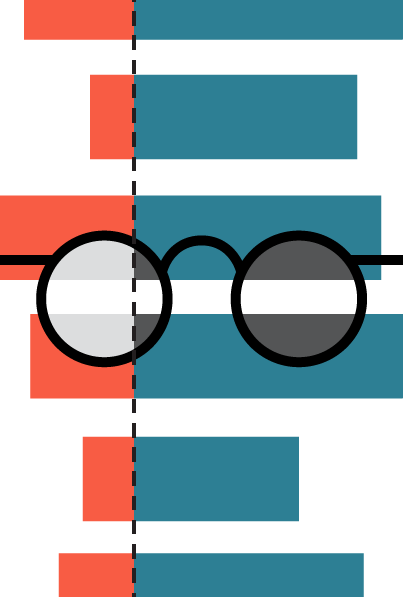
\includegraphics{data-vis-tips.png}

}

\caption{\label{fig-kitty}Frequency distribution shapes}

\end{figure}%

Figure~\ref{fig-plot} demonstrates interactive components for graphical
representations of data. In presentations, this may be helpful to
reinforce scale(s) of measurement, obtain feedback on data clusters, and
highlight differences between aggregate and individual datapoints.

\begin{figure}

\centering{

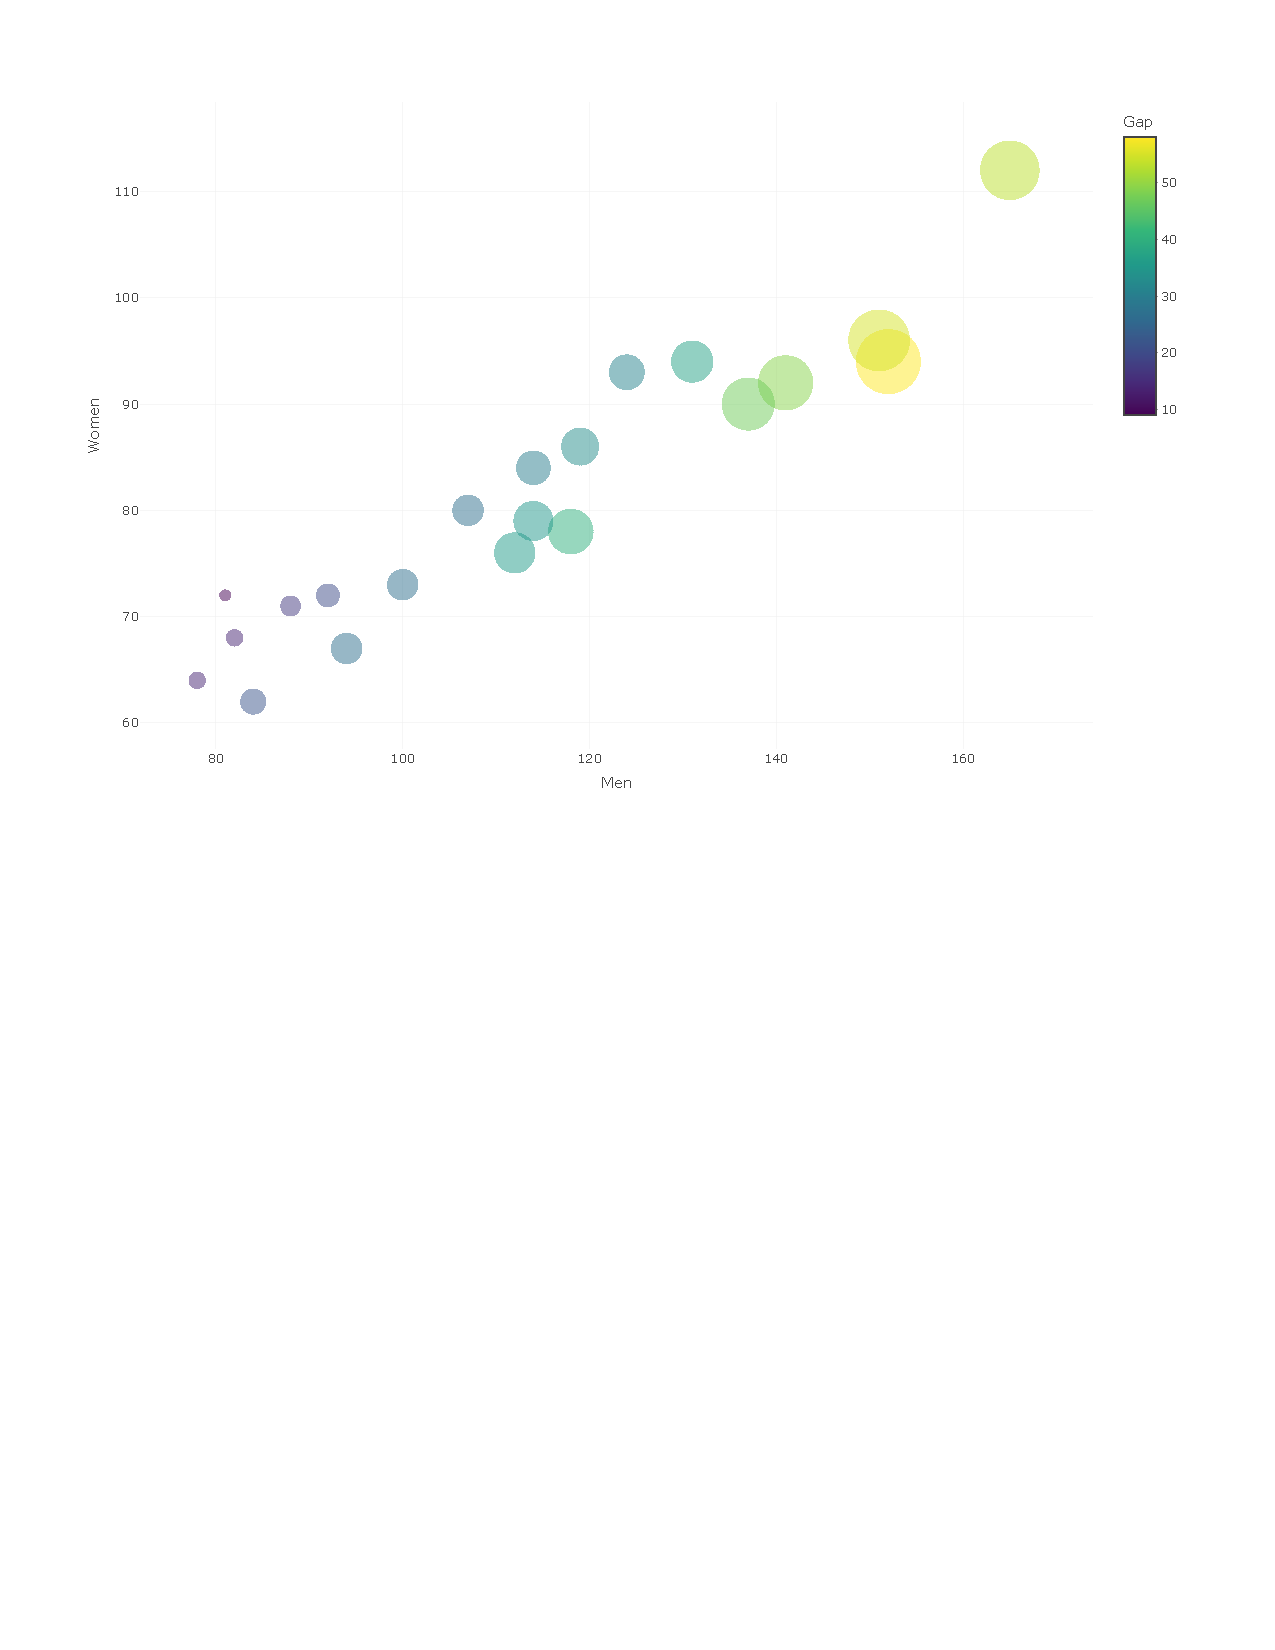
\includegraphics{summary_files/figure-pdf/fig-plot-1.pdf}

}

\caption{\label{fig-plot}Example interactive plot}

\end{figure}%

\section{Geo-spatial}\label{geo-spatial}

Figure~\ref{fig-map} is another example of interactivity - a map such as
this can help reinforce viewer concepts such as
\emph{representativeness} within normative samples (e.g., where the data
``came from'' and who the data represents).

\begin{tcolorbox}[enhanced jigsaw, colbacktitle=quarto-callout-note-color!10!white, coltitle=black, rightrule=.15mm, toprule=.15mm, left=2mm, arc=.35mm, colframe=quarto-callout-note-color-frame, opacityback=0, breakable, bottomrule=.15mm, bottomtitle=1mm, opacitybacktitle=0.6, toptitle=1mm, titlerule=0mm, title=\textcolor{quarto-callout-note-color}{\faInfo}\hspace{0.5em}{Browsers vs.~Static PDF Readers}, leftrule=.75mm, colback=white]

Note that all interactive visuals will be captured via static
representation if a reader elects to download a PDF file (by accessing
the button located within the toolbar). These images are not currently
optimized for static representation, so interactivity will render
imperfectly within the example PDF.

\end{tcolorbox}

\begin{figure}

\centering{

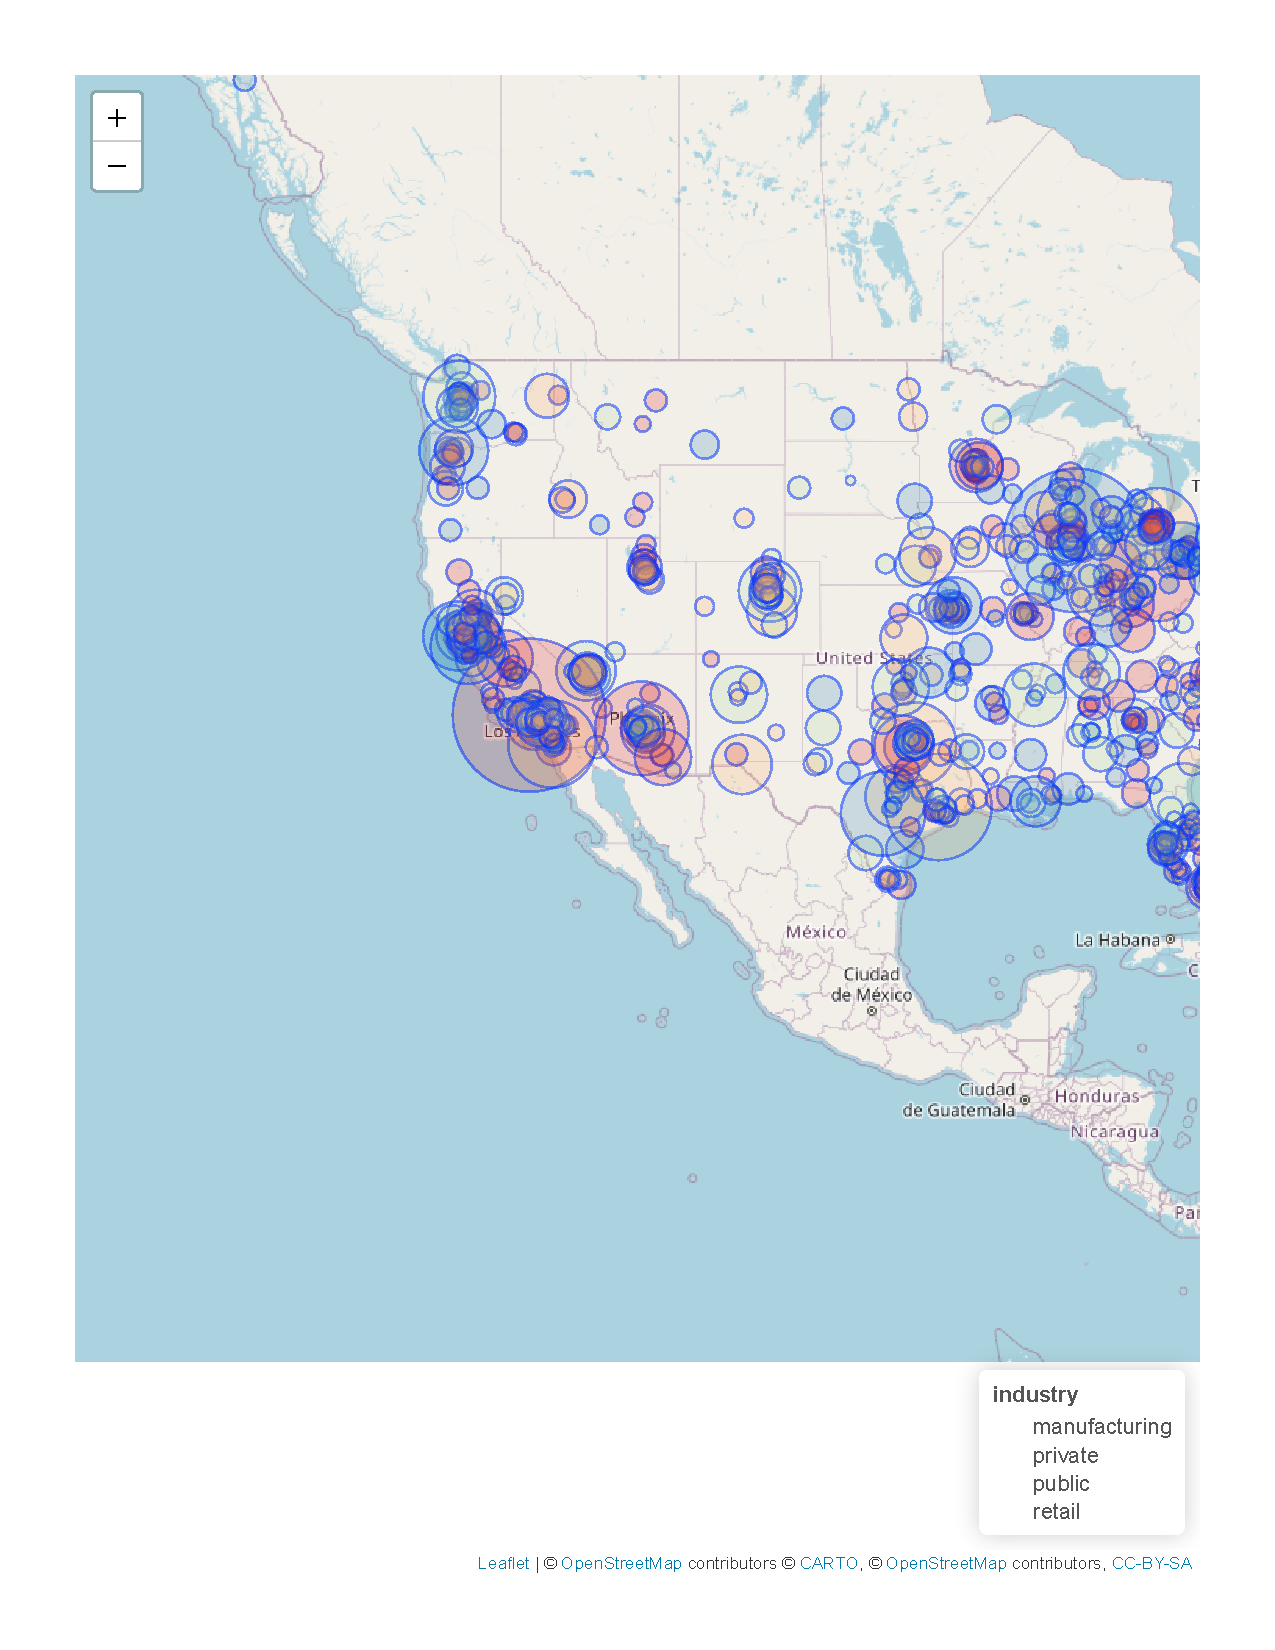
\includegraphics{summary_files/figure-pdf/fig-map-1.pdf}

}

\caption{\label{fig-map}Example normative representation by geographic
location.}

\end{figure}%

\section{Multi-media}\label{multi-media}

Figure~\ref{fig-pink} shows yet another example - videos can be pulled
from external sites (like this presentation of using

\includegraphics[width=1.13em,height=1em]{summary_files/figure-pdf/fa-icon-4912d291b82ba7bbcd2aacb159b216f4.pdf}
to create and deploy organizational surveys) or can present locally
produced video files.

\begin{figure}

\centering{

\url{https://www.youtube.com/watch?v=GgW87oQKGQ8&t=630s}

}

\caption{\label{fig-pink}Using

\includegraphics[width=1.13em,height=1em]{summary_files/figure-pdf/fa-icon-4912d291b82ba7bbcd2aacb159b216f4.pdf}
to design, deploy, and store survey data}

\end{figure}%

\bookmarksetup{startatroot}

\chapter{Code Access}\label{code-access}

As a practitioner of data science principles, your code Error is
minimized by incorporating your analyses within your documentation. The
two processes

Hyperlinks connect content both within and external to the book material
(for example, citations; See Knuth (1984) for an early discussion of
literate programming {[}the underlying philosophy driving this authoring
platform{]}). Or, see Chapter~\ref{sec-summary} for a demonstration of
image and figure capabilities.

\section{Code sharing}\label{code-sharing}

The underlying statistical languages represent one source of error
within presentations of data analysis. Literate programming authoring
platforms offer several features intended to provide full transparency
to the process(es) used to conduct an analysis.

The code represented in Listing~\ref{lst-first} (and all example pieces
of code) can be copied by activating the clipboard option in the
upper-right hand corner of the code chunk.

\begin{tcolorbox}[enhanced jigsaw, colbacktitle=quarto-callout-tip-color!10!white, coltitle=black, rightrule=.15mm, toprule=.15mm, left=2mm, arc=.35mm, colframe=quarto-callout-tip-color-frame, opacityback=0, breakable, bottomrule=.15mm, bottomtitle=1mm, opacitybacktitle=0.6, toptitle=1mm, titlerule=0mm, title=\textcolor{quarto-callout-tip-color}{\faLightbulb}\hspace{0.5em}{Tip}, leftrule=.75mm, colback=white]

\texttt{R} code can always be copied onto your personal computer via the
clipboard icon:

\includegraphics[width=0.75em,height=1em]{intro_files/figure-pdf/fa-icon-9dbb28eb5af36d9fcb6d2e28bc0a04a4.pdf}.

\end{tcolorbox}

\begin{codelisting}

\caption{\label{lst-first}Addition within \texttt{R}}

\centering{

\begin{Shaded}
\begin{Highlighting}[]
\DecValTok{1} \SpecialCharTok{+} \DecValTok{1}                                    
\end{Highlighting}
\end{Shaded}

}

\end{codelisting}%

For more complex bits of analysis, hidden annotations are available (the
audience can further access notes/assistance by hovering over the
circled numbers):

\phantomsection\label{lst-second}%
\begin{Shaded}
\begin{Highlighting}[]
\FunctionTok{library}\NormalTok{(psych) }\hspace*{\fill}\NormalTok{\circled{1}}
\FunctionTok{data}\NormalTok{(bfi) }\hspace*{\fill}\NormalTok{\circled{2}}

\NormalTok{bfi}\SpecialCharTok{$}\NormalTok{jibberish }\OtherTok{\textless{}{-}} \FunctionTok{rowMeans}\NormalTok{(bfi[}\DecValTok{1}\SpecialCharTok{:}\DecValTok{10}\NormalTok{], }\AttributeTok{na.rm=}\ConstantTok{TRUE}\NormalTok{) }\hspace*{\fill}\NormalTok{\circled{3}}
\NormalTok{bfi}\SpecialCharTok{$}\NormalTok{gobbleyjook }\OtherTok{\textless{}{-}} \FunctionTok{rowMeans}\NormalTok{(bfi[}\DecValTok{11}\SpecialCharTok{:}\DecValTok{20}\NormalTok{], }\AttributeTok{na.rm=}\ConstantTok{TRUE}\NormalTok{) }
\end{Highlighting}
\end{Shaded}

\begin{description}
\tightlist
\item[\circled{1}]
The \texttt{psych} package contains example data that we can access.
\item[\circled{2}]
This gives us access to the \texttt{bfi} dataset that contains
personality item responses.
\item[\circled{3}]
We make 2 scale scores, \texttt{jibberish} and \texttt{gobbleyjook}. The
\texttt{\$} notation indicates that these scale scores will be appended
to the \texttt{bfi} dataframe.
\end{description}

The entire code block can also be hidden unless asked-for\footnote{In
  html format only.}. These features permit students of different
knowledge and confidence levels to access help on an as-needed basis:

\phantomsection\label{lst-three}%
\begin{Shaded}
\begin{Highlighting}[]
\FunctionTok{library}\NormalTok{(psych) }\hspace*{\fill}\NormalTok{\circled{1}}
\FunctionTok{data}\NormalTok{(bfi) }\hspace*{\fill}\NormalTok{\circled{2}}

\NormalTok{bfi}\SpecialCharTok{$}\NormalTok{jibberish }\OtherTok{\textless{}{-}} \FunctionTok{rowMeans}\NormalTok{(bfi[}\DecValTok{1}\SpecialCharTok{:}\DecValTok{10}\NormalTok{], }\AttributeTok{na.rm=}\ConstantTok{TRUE}\NormalTok{) }\hspace*{\fill}\NormalTok{\circled{3}}
\NormalTok{bfi}\SpecialCharTok{$}\NormalTok{gobbleyjook }\OtherTok{\textless{}{-}} \FunctionTok{rowMeans}\NormalTok{(bfi[}\DecValTok{11}\SpecialCharTok{:}\DecValTok{20}\NormalTok{], }\AttributeTok{na.rm=}\ConstantTok{TRUE}\NormalTok{) }
\end{Highlighting}
\end{Shaded}

\begin{description}
\tightlist
\item[\circled{1}]
The \texttt{psych} package contains example data that we can access.
\item[\circled{2}]
This gives us access to the \texttt{bfi} dataset that contains
personality item responses.
\item[\circled{3}]
We make 2 scale scores, \texttt{jibberish} and \texttt{gobbleyjook}. The
\texttt{\$} notation indicates that these scale scores will be appended
to the \texttt{bfi} dataframe.
\end{description}

\bookmarksetup{startatroot}

\chapter{Platforms}\label{platforms}

You can author within any text editor (including, for example, Windows-
or Mac-based editors such as \texttt{notepad} or \texttt{TextEdit}).
However, most content creators prefer to use an integrated development
environment (IDE). Popular IDEs that facilitate literate programming
across languages (e.g., R/Python) include:

\begin{itemize}
\tightlist
\item
  \href{https://posit.co/download/rstudio-desktop/}{RStudio}
\item
  Visual Studio Code (aka \href{https://code.visualstudio.com/}{VS
  Code})
\item
  \href{https://positron.posit.co/}{Positron}
\end{itemize}

Note that there are very many possible IDEs to use as of
\texttt{r\ format(Sys.time(),\ "\%B\ \%Y")} -- your choice of IDE is not
limited to these above-listed options. If you prefer a different
IDE\footnote{for example, if you intend to only use Python as an
  analytical language and are already comfortable using \texttt{Jupyter}
  or \texttt{Spyder}}, please let the instructor know so he/she can:

\begin{enumerate}
\def\labelenumi{\arabic{enumi}.}
\tightlist
\item
  better assist you, and
\item
  (very likely) learn about an alternative IDE
\end{enumerate}

\subsection{RStudio}\label{rstudio}

\subsection{VS Code}\label{vs-code}

\subsection{Positron}\label{positron}

\bookmarksetup{startatroot}

\chapter*{References}\label{references}
\addcontentsline{toc}{chapter}{References}

\markboth{References}{References}

\phantomsection\label{refs}
\begin{CSLReferences}{1}{0}
\bibitem[\citeproctext]{ref-knuth84}
Knuth, Donald E. 1984. {``Literate Programming.''} \emph{Comput. J.} 27
(2): 97--111. \url{https://doi.org/10.1093/comjnl/27.2.97}.

\end{CSLReferences}




\end{document}
